% Graphic for TeX using PGF
% Title: /home/maximilien/INSA/alambic/report/draw/uml_completion_structure.dia
% Creator: Dia v0.97.3
% CreationDate: Sun Apr 19 22:18:30 2015
% For: maximilien
% \usepackage{tikz}
% The following commands are not supported in PSTricks at present
% We define them conditionally, so when they are implemented,
% this pgf file will use them.
\ifx\du\undefined
  \newlength{\du}
\fi
\setlength{\du}{15\unitlength}
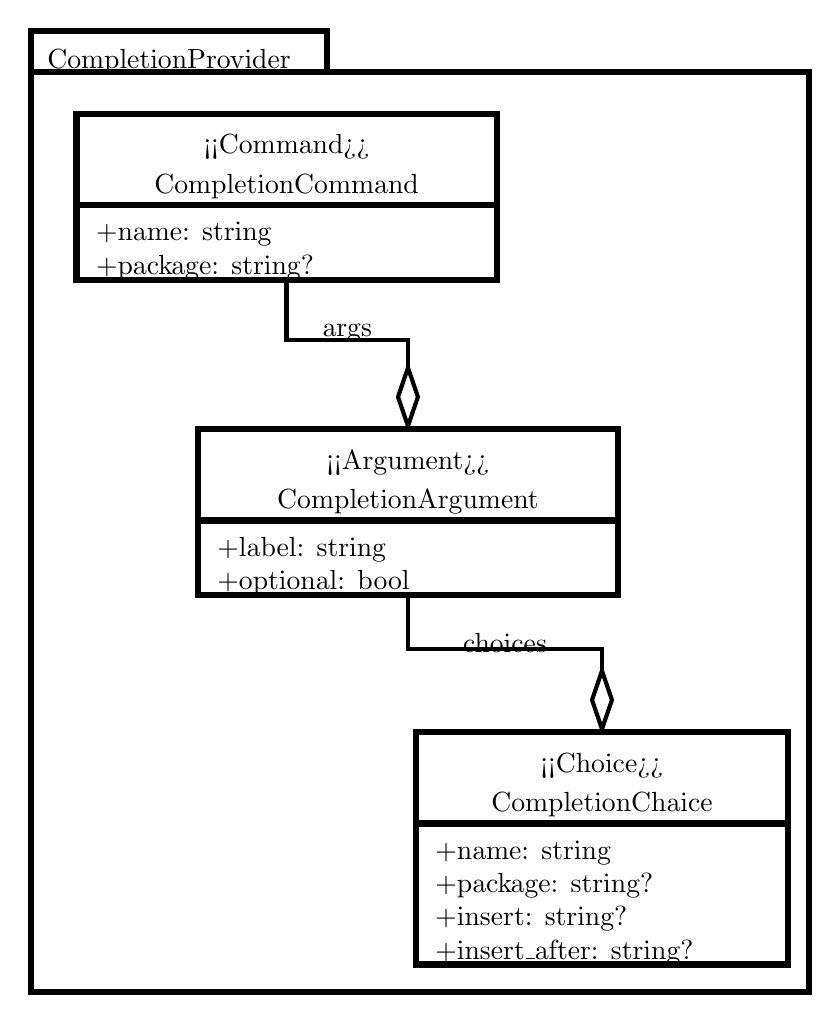
\begin{tikzpicture}
\pgftransformxscale{1.000000}
\pgftransformyscale{-1.000000}
\definecolor{dialinecolor}{rgb}{0.000000, 0.000000, 0.000000}
\pgfsetstrokecolor{dialinecolor}
\definecolor{dialinecolor}{rgb}{1.000000, 1.000000, 1.000000}
\pgfsetfillcolor{dialinecolor}
\pgfsetlinewidth{0.150000\du}
\pgfsetdash{}{0pt}
\definecolor{dialinecolor}{rgb}{1.000000, 1.000000, 1.000000}
\pgfsetfillcolor{dialinecolor}
\fill (1.100000\du,1.450000\du)--(1.100000\du,23.600000\du)--(19.850000\du,23.600000\du)--(19.850000\du,1.450000\du)--cycle;
\definecolor{dialinecolor}{rgb}{0.000000, 0.000000, 0.000000}
\pgfsetstrokecolor{dialinecolor}
\draw (1.100000\du,1.450000\du)--(1.100000\du,23.600000\du)--(19.850000\du,23.600000\du)--(19.850000\du,1.450000\du)--cycle;
\definecolor{dialinecolor}{rgb}{1.000000, 1.000000, 1.000000}
\pgfsetfillcolor{dialinecolor}
\fill (1.100000\du,0.450000\du)--(1.100000\du,1.450000\du)--(8.230000\du,1.450000\du)--(8.230000\du,0.450000\du)--cycle;
\definecolor{dialinecolor}{rgb}{0.000000, 0.000000, 0.000000}
\pgfsetstrokecolor{dialinecolor}
\draw (1.100000\du,0.450000\du)--(1.100000\du,1.450000\du)--(8.230000\du,1.450000\du)--(8.230000\du,0.450000\du)--cycle;
% setfont left to latex
\definecolor{dialinecolor}{rgb}{0.000000, 0.000000, 0.000000}
\pgfsetstrokecolor{dialinecolor}
\node[anchor=west] at (1.200000\du,1.200000\du){CompletionProvider};
\pgfsetlinewidth{0.150000\du}
\pgfsetdash{}{0pt}
\definecolor{dialinecolor}{rgb}{1.000000, 1.000000, 1.000000}
\pgfsetfillcolor{dialinecolor}
\fill (2.200000\du,2.450000\du)--(2.200000\du,4.650000\du)--(12.322500\du,4.650000\du)--(12.322500\du,2.450000\du)--cycle;
\definecolor{dialinecolor}{rgb}{0.000000, 0.000000, 0.000000}
\pgfsetstrokecolor{dialinecolor}
\draw (2.200000\du,2.450000\du)--(2.200000\du,4.650000\du)--(12.322500\du,4.650000\du)--(12.322500\du,2.450000\du)--cycle;
% setfont left to latex
\definecolor{dialinecolor}{rgb}{0.000000, 0.000000, 0.000000}
\pgfsetstrokecolor{dialinecolor}
\node at (7.261250\du,3.250000\du){<<Command>>};
% setfont left to latex
\definecolor{dialinecolor}{rgb}{0.000000, 0.000000, 0.000000}
\pgfsetstrokecolor{dialinecolor}
\node at (7.261250\du,4.200000\du){CompletionCommand};
\definecolor{dialinecolor}{rgb}{1.000000, 1.000000, 1.000000}
\pgfsetfillcolor{dialinecolor}
\fill (2.200000\du,4.650000\du)--(2.200000\du,6.450000\du)--(12.322500\du,6.450000\du)--(12.322500\du,4.650000\du)--cycle;
\definecolor{dialinecolor}{rgb}{0.000000, 0.000000, 0.000000}
\pgfsetstrokecolor{dialinecolor}
\draw (2.200000\du,4.650000\du)--(2.200000\du,6.450000\du)--(12.322500\du,6.450000\du)--(12.322500\du,4.650000\du)--cycle;
% setfont left to latex
\definecolor{dialinecolor}{rgb}{0.000000, 0.000000, 0.000000}
\pgfsetstrokecolor{dialinecolor}
\node[anchor=west] at (2.375000\du,5.350000\du){+name: string};
% setfont left to latex
\definecolor{dialinecolor}{rgb}{0.000000, 0.000000, 0.000000}
\pgfsetstrokecolor{dialinecolor}
\node[anchor=west] at (2.375000\du,6.150000\du){+package: string?};
\pgfsetlinewidth{0.150000\du}
\pgfsetdash{}{0pt}
\definecolor{dialinecolor}{rgb}{1.000000, 1.000000, 1.000000}
\pgfsetfillcolor{dialinecolor}
\fill (5.125000\du,10.045000\du)--(5.125000\du,12.245000\du)--(15.247500\du,12.245000\du)--(15.247500\du,10.045000\du)--cycle;
\definecolor{dialinecolor}{rgb}{0.000000, 0.000000, 0.000000}
\pgfsetstrokecolor{dialinecolor}
\draw (5.125000\du,10.045000\du)--(5.125000\du,12.245000\du)--(15.247500\du,12.245000\du)--(15.247500\du,10.045000\du)--cycle;
% setfont left to latex
\definecolor{dialinecolor}{rgb}{0.000000, 0.000000, 0.000000}
\pgfsetstrokecolor{dialinecolor}
\node at (10.186250\du,10.845000\du){<<Argument>>};
% setfont left to latex
\definecolor{dialinecolor}{rgb}{0.000000, 0.000000, 0.000000}
\pgfsetstrokecolor{dialinecolor}
\node at (10.186250\du,11.795000\du){CompletionArgument};
\definecolor{dialinecolor}{rgb}{1.000000, 1.000000, 1.000000}
\pgfsetfillcolor{dialinecolor}
\fill (5.125000\du,12.245000\du)--(5.125000\du,14.045000\du)--(15.247500\du,14.045000\du)--(15.247500\du,12.245000\du)--cycle;
\definecolor{dialinecolor}{rgb}{0.000000, 0.000000, 0.000000}
\pgfsetstrokecolor{dialinecolor}
\draw (5.125000\du,12.245000\du)--(5.125000\du,14.045000\du)--(15.247500\du,14.045000\du)--(15.247500\du,12.245000\du)--cycle;
% setfont left to latex
\definecolor{dialinecolor}{rgb}{0.000000, 0.000000, 0.000000}
\pgfsetstrokecolor{dialinecolor}
\node[anchor=west] at (5.300000\du,12.945000\du){+label: string};
% setfont left to latex
\definecolor{dialinecolor}{rgb}{0.000000, 0.000000, 0.000000}
\pgfsetstrokecolor{dialinecolor}
\node[anchor=west] at (5.300000\du,13.745000\du){+optional: bool};
\pgfsetlinewidth{0.100000\du}
\pgfsetdash{}{0pt}
\pgfsetmiterjoin
\pgfsetbuttcap
{
\definecolor{dialinecolor}{rgb}{0.000000, 0.000000, 0.000000}
\pgfsetfillcolor{dialinecolor}
% was here!!!
\definecolor{dialinecolor}{rgb}{0.000000, 0.000000, 0.000000}
\pgfsetstrokecolor{dialinecolor}
\draw (10.186250\du,9.969747\du)--(10.186250\du,7.897500\du)--(7.261250\du,7.897500\du)--(7.261250\du,6.525253\du);
}
\definecolor{dialinecolor}{rgb}{0.000000, 0.000000, 0.000000}
\pgfsetstrokecolor{dialinecolor}
\draw (10.186250\du,8.711168\du)--(10.186250\du,7.897500\du)--(7.261250\du,7.897500\du)--(7.261250\du,6.525253\du);
\pgfsetdash{}{0pt}
\pgfsetmiterjoin
\pgfsetbuttcap
\definecolor{dialinecolor}{rgb}{1.000000, 1.000000, 1.000000}
\pgfsetfillcolor{dialinecolor}
\fill (10.186250\du,9.969747\du)--(9.946250\du,9.269747\du)--(10.186250\du,8.569747\du)--(10.426250\du,9.269747\du)--cycle;
\pgfsetlinewidth{0.100000\du}
\pgfsetdash{}{0pt}
\pgfsetmiterjoin
\pgfsetbuttcap
\definecolor{dialinecolor}{rgb}{0.000000, 0.000000, 0.000000}
\pgfsetstrokecolor{dialinecolor}
\draw (10.186250\du,9.969747\du)--(9.946250\du,9.269747\du)--(10.186250\du,8.569747\du)--(10.426250\du,9.269747\du)--cycle;
% setfont left to latex
\definecolor{dialinecolor}{rgb}{0.000000, 0.000000, 0.000000}
\pgfsetstrokecolor{dialinecolor}
\node at (8.723750\du,7.747500\du){args};
\pgfsetlinewidth{0.150000\du}
\pgfsetdash{}{0pt}
\definecolor{dialinecolor}{rgb}{1.000000, 1.000000, 1.000000}
\pgfsetfillcolor{dialinecolor}
\fill (10.375000\du,17.345000\du)--(10.375000\du,19.545000\du)--(19.345000\du,19.545000\du)--(19.345000\du,17.345000\du)--cycle;
\definecolor{dialinecolor}{rgb}{0.000000, 0.000000, 0.000000}
\pgfsetstrokecolor{dialinecolor}
\draw (10.375000\du,17.345000\du)--(10.375000\du,19.545000\du)--(19.345000\du,19.545000\du)--(19.345000\du,17.345000\du)--cycle;
% setfont left to latex
\definecolor{dialinecolor}{rgb}{0.000000, 0.000000, 0.000000}
\pgfsetstrokecolor{dialinecolor}
\node at (14.860000\du,18.145000\du){<<Choice>>};
% setfont left to latex
\definecolor{dialinecolor}{rgb}{0.000000, 0.000000, 0.000000}
\pgfsetstrokecolor{dialinecolor}
\node at (14.860000\du,19.095000\du){CompletionChaice};
\definecolor{dialinecolor}{rgb}{1.000000, 1.000000, 1.000000}
\pgfsetfillcolor{dialinecolor}
\fill (10.375000\du,19.545000\du)--(10.375000\du,22.945000\du)--(19.345000\du,22.945000\du)--(19.345000\du,19.545000\du)--cycle;
\definecolor{dialinecolor}{rgb}{0.000000, 0.000000, 0.000000}
\pgfsetstrokecolor{dialinecolor}
\draw (10.375000\du,19.545000\du)--(10.375000\du,22.945000\du)--(19.345000\du,22.945000\du)--(19.345000\du,19.545000\du)--cycle;
% setfont left to latex
\definecolor{dialinecolor}{rgb}{0.000000, 0.000000, 0.000000}
\pgfsetstrokecolor{dialinecolor}
\node[anchor=west] at (10.550000\du,20.245000\du){+name: string};
% setfont left to latex
\definecolor{dialinecolor}{rgb}{0.000000, 0.000000, 0.000000}
\pgfsetstrokecolor{dialinecolor}
\node[anchor=west] at (10.550000\du,21.045000\du){+package: string?};
% setfont left to latex
\definecolor{dialinecolor}{rgb}{0.000000, 0.000000, 0.000000}
\pgfsetstrokecolor{dialinecolor}
\node[anchor=west] at (10.550000\du,21.845000\du){+insert: string?};
% setfont left to latex
\definecolor{dialinecolor}{rgb}{0.000000, 0.000000, 0.000000}
\pgfsetstrokecolor{dialinecolor}
\node[anchor=west] at (10.550000\du,22.645000\du){+insert\_after: string?};
\pgfsetlinewidth{0.100000\du}
\pgfsetdash{}{0pt}
\pgfsetmiterjoin
\pgfsetbuttcap
{
\definecolor{dialinecolor}{rgb}{0.000000, 0.000000, 0.000000}
\pgfsetfillcolor{dialinecolor}
% was here!!!
\definecolor{dialinecolor}{rgb}{0.000000, 0.000000, 0.000000}
\pgfsetstrokecolor{dialinecolor}
\draw (14.860000\du,17.269649\du)--(14.860000\du,15.344951\du)--(10.186250\du,15.344951\du)--(10.186250\du,14.120253\du);
}
\definecolor{dialinecolor}{rgb}{0.000000, 0.000000, 0.000000}
\pgfsetstrokecolor{dialinecolor}
\draw (14.860000\du,16.011070\du)--(14.860000\du,15.344951\du)--(10.186250\du,15.344951\du)--(10.186250\du,14.120253\du);
\pgfsetdash{}{0pt}
\pgfsetmiterjoin
\pgfsetbuttcap
\definecolor{dialinecolor}{rgb}{1.000000, 1.000000, 1.000000}
\pgfsetfillcolor{dialinecolor}
\fill (14.860000\du,17.269649\du)--(14.620000\du,16.569649\du)--(14.860000\du,15.869649\du)--(15.100000\du,16.569649\du)--cycle;
\pgfsetlinewidth{0.100000\du}
\pgfsetdash{}{0pt}
\pgfsetmiterjoin
\pgfsetbuttcap
\definecolor{dialinecolor}{rgb}{0.000000, 0.000000, 0.000000}
\pgfsetstrokecolor{dialinecolor}
\draw (14.860000\du,17.269649\du)--(14.620000\du,16.569649\du)--(14.860000\du,15.869649\du)--(15.100000\du,16.569649\du)--cycle;
% setfont left to latex
\definecolor{dialinecolor}{rgb}{0.000000, 0.000000, 0.000000}
\pgfsetstrokecolor{dialinecolor}
\node at (12.523125\du,15.194951\du){choices};
\end{tikzpicture}
